\section{Methodology}
\label{sec:methodology}

\subsection{Construction of the Sketch}
Metadata extraction and organization

Fine-grained/coarse-grained representations

Dynamic reorientations of the graph

Representativeness across time intervals

\subsection{Stream Partitioning}
We use the Geohash~algorithm~\cite{geohash} to balance load and partition incoming data streams across processing resources. Geohash divides the earth into a hierarchy of bounding boxes identified by Base 32 strings; the longer the Geohash string, the more precise the bounding box. Figure~\ref{fig:geohash} illustrates this hierarchy; most of the western United States and Mexico are contained within the bounding box described by Geohash string \emph{9}, while \emph{9Q} encompasses parts of California, Nevada, Arizona, and Utah. The bounding box \emph{9Q9K} (highlighted in red) contains San Jose, California. This hierarchical representation enables \textsc{Rivulet} to cope with both low- and high-density regions. For instance, several resources may be tasked with managing streams originating in and around the San Francisco region, while the entirety of Yosemite National Park could fall under the purview of a single node.

\begin{figure}
    \centerline{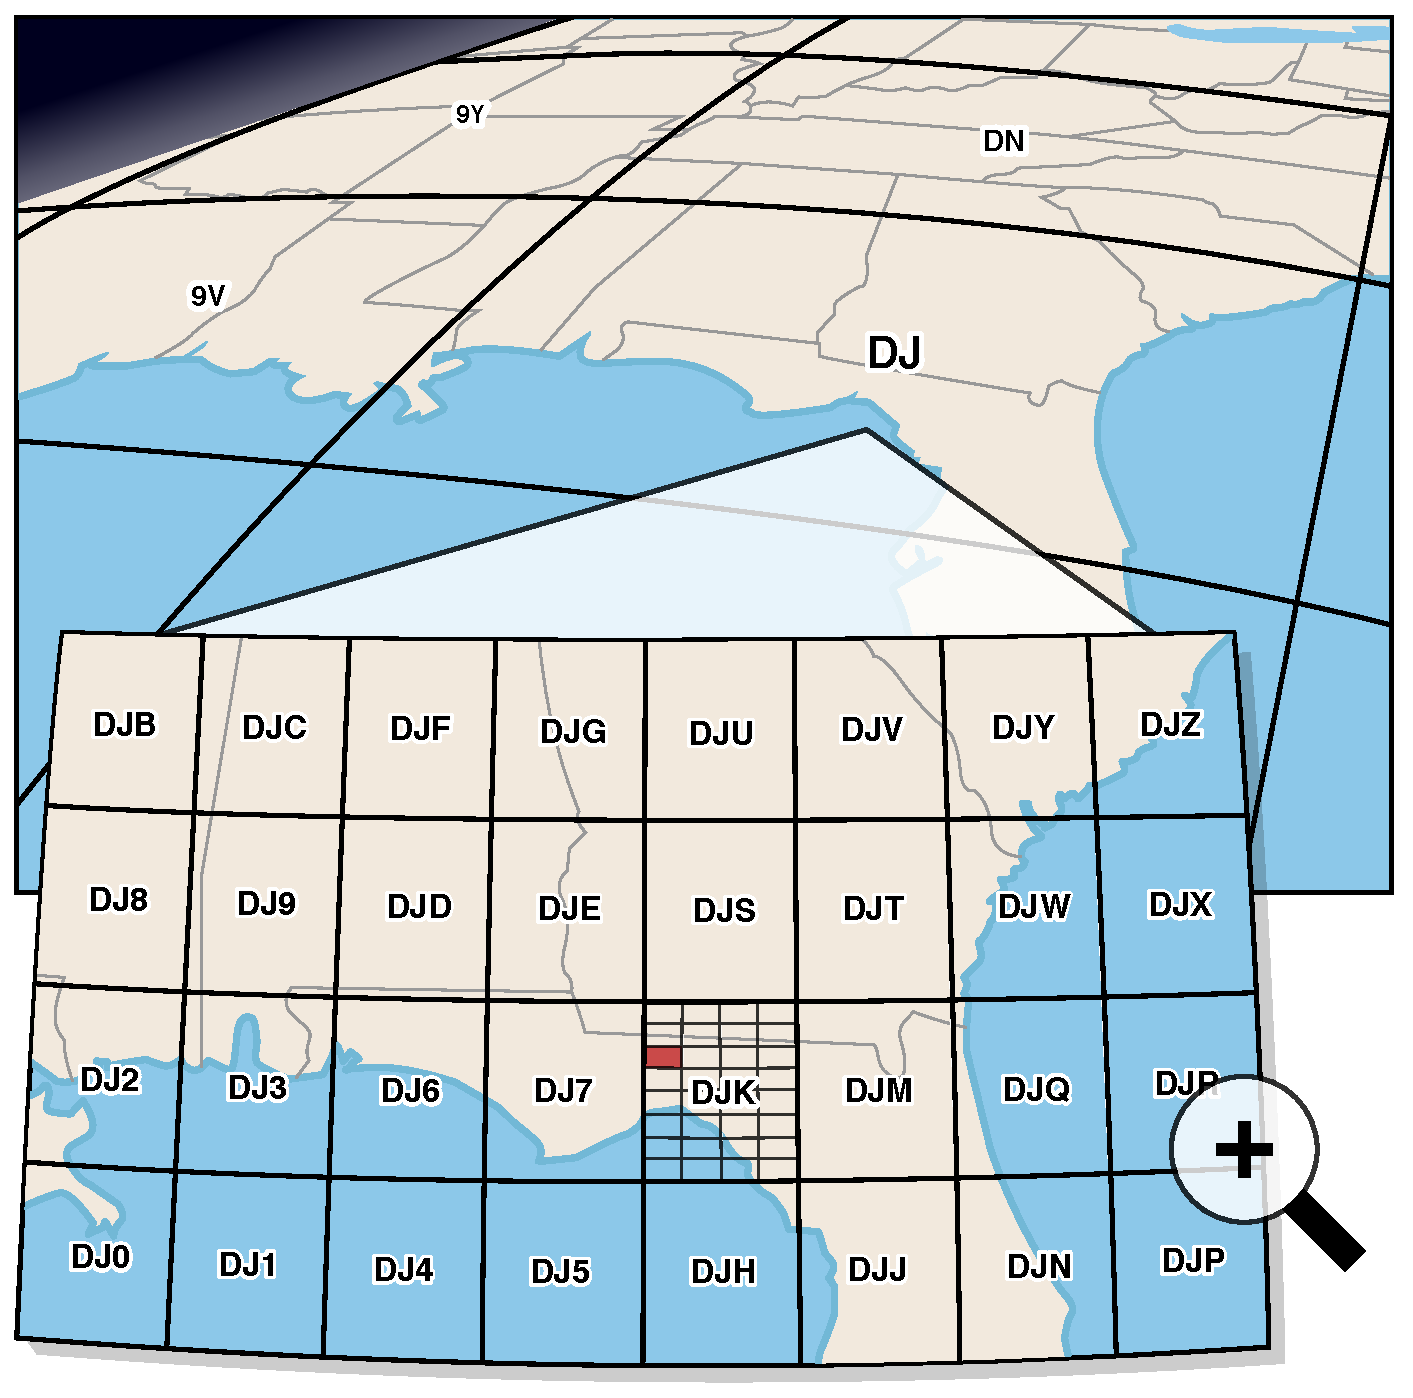
\includegraphics[width=3.5in]{figures/geohash.pdf}}
    \caption{A demonstration of the Geohash algorithm. Each additional character in a Geohash string describes a finer-grained region; Geohash \emph{9Q} contains a substantial portion of California, USA, while \emph{9Q9K} (highlighted in red) represents a smaller region containing San Jose, California.}
    \label{fig:geohash}
\end{figure}

To achieve fine-grained control over our Geohash partitions, we operate at the bit level rather than Base 32 character level when routing streams. Each bit added to a Geohash string reduces its scope by half, with each character represented by five bits ($2^5 = 32$). In other words, a four-character Geohash string represents 20 spatial subdivisions. This property allows us to manage and allocate resources across a wide variety of observational densities.

 % This needs to be moved as we get the paper structure finalized

\subsection{Coping with High Data Rates: Scaling out}
\begin{figure}
    \centerline{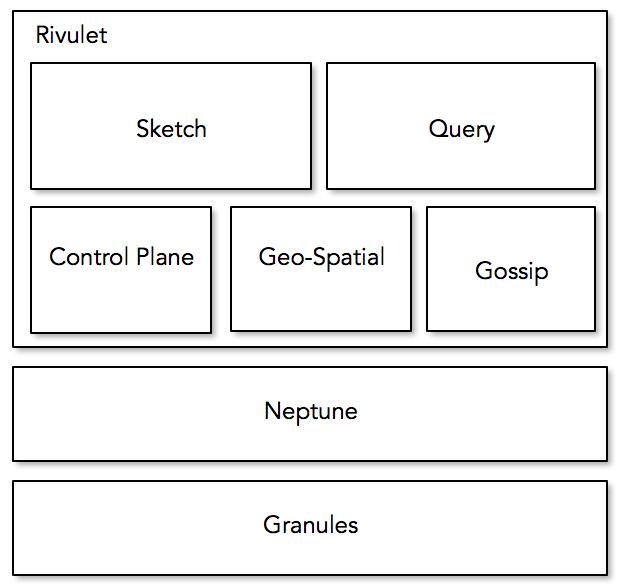
\includegraphics[scale=0.5]{figures/rivulet-archi.png}}
    \caption{Rivulet is implemented as a specialized layer for geo-spatial data on top of Neptune stream processing system..}
    \label{fig:process-monitor}
\end{figure}
%
\begin{figure}
    \centerline{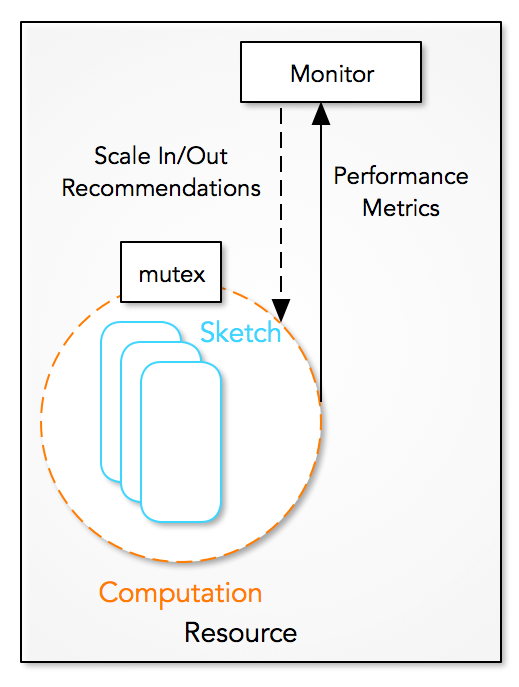
\includegraphics[scale=0.55]{figures/process-monitor.png}}
    \caption{Dynamic scaling is triggered by monitoring the backlog of each computation and memory pressure incurred in each process.}
    \label{fig:process-monitor}
\end{figure}
%
\begin{figure}
    \centerline{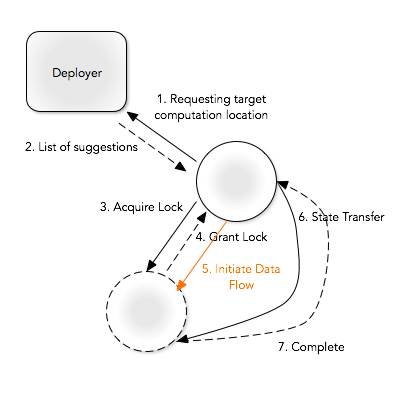
\includegraphics[scale=0.55]{figures/scale-out-protocol.png}}
    \caption{Scale out protocol}
    \label{fig:scale-out-protocol}
\end{figure}
%
\subsection{Downscaling}
\begin{figure}
    \centerline{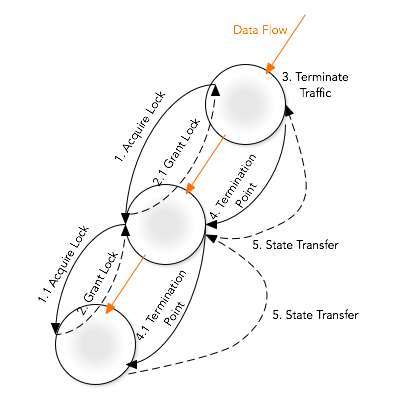
\includegraphics[scale=0.55]{figures/scale-in-protocol.png}}
    \caption{Scale in protocol}
    \label{fig:scale-in-protocol}
\end{figure}

\subsection{Query Evaluations}
Accounting for data arrival rates, accuracy requirements, memory pressures, and the capacity of network links result in dynamic upscaling and downscaling of nodes that comprise Rivulet. The result of these scaling operations is a distributed sketch, with constituent nodes holding compact representations of observational data from different geographic locations. 

Information about nodes that comprise the Rivulet sketch is maintained as a prefix tree at each node. Addition and removal of nodes comprising the distributed sketch due to scaling maneuvers are propagated through the system and the prefix trees updated. Information within the prefix trees is designed to be eventually consistent.  Alongside each vertex in this prefix tree, we maintain information about the spatiotemporal scope/range and the set of features available at the node.  

Rivulet incorporates support for discrete and continuous queries specified by users. Queries specified by a user are evaluated over the distributed sketch. Depending on the spatial scopes that may be implicitly or explicitly specified within these queries, query evaluations will be performed on one or more nodes comprising the distributed sketch. 

The entry point for these queries may be any of the nodes comprising the distributed sketch – we refer to this node as the conduit for the particular query.  During query evaluations, a first step is to identify the set of Rivulet nodes that must be targeted for query evaluations. The conduit node consults its prefix tree to identify nodes to contact based on the spatial, chronological, and particular features implied in the query. Conduit nodes are responsible for forwarding queries to the relevant nodes comprising the distributed sketch where the query must be evaluated.  The conduit node also responds to the client with the list of nodes that will be responding to the query. 

Results from query evaluations performed over the distributed sketch are streamed back to the client.  Precisely what is streamed depends on the nature of the query.  For example, if a client is interested in retrieving average temperatures in Colorado for July 2015 and if there are multiple nodes (within Rivulet) that hold relevant portions of this data; then the query must be forwarded to all these nodes. The results returned from each of these nodes would include {\textless}temperature, frequency{\textgreater} tuples that would then be combined at the client side to compute the final average temperature.

Alternatively, Rivulet nodes participating in the query evaluations will return vertices and edges (from their internal sketches) that satisfied the specified query constraints. The vertices and edges will be restricted to those pertinent to the query. For example, if a query targets a particular feature (say humidity) then vertices/edges relating to other features not targeted by the query will be pruned and not returned.  Spatiotemporal features are exempt from this constraint. As vertices and edges are streamed back to the client from multiple nodes comprising Rivulet, these are organized into a graph that is then used to return the final results. 

The prefix tree also allows query evaluations during both upscaling and downscaling operations. During query evaluations, queries are forwarded to child nodes (created during a recent upscaling operation). When the conduit forwards a query to a Rivulet node and the node is unavailable, it is either due to a failure at that node or a downscaling operation that merges the child node with its parent node. When a node is unreachable, the conduit forwards the query to the parent node. 

\subsection{Types of Queries}
Queries within Rivulet can be discrete or continuous queries. Unlike discrete queries that are evaluated once, continuous queries are evaluated periodically or when observations become available. Though observations are never stored on stable storage, queries specified by users may target spatial and chronological scopes. In the case of continuous queries, the chronological range implicitly evolves as new observations trickle in; in the case of windowing operators, the specified chronological window continually slides over the observational streams. We classify queries – discrete or continuous –   supported by Rivulet into 5 broad queries. These include:
\begin{enumerate} 
	\item	Filter queries that specify inequality/relational queries along one or more dimensions. 
	\item	Statistical queries allow users to explore statistical properties of the observational space. For example, users can retrieve and contrast correlations between any two features at different geographic locations at the same time. Alternatively, queries may contrast correlations between different features at different time ranges at the same geographic location. Statistical queries also support retrieval of the mean, standard deviation, and also of feature outliers based on Chebyshev’s rule about the distribution of feature values.
	\item	Density queries support analysis over the distribution of values associated with a feature over a particular spatiotemporal scope. These include kernel density estimations, estimating the probability of observing a particular value for an observation, and determining the deciles and quartiles for the observed feature. 
	\item	Set Queries target identification of whether a particular combination of feature values was observed, estimating the cardinality of the dataset, and identifying the frequencies of repeated observations.
	\item	Inferential queries are intended to support projections about how the feature is expected to evolve over a spatiotemporal scope. In this study, these projections are predicated on the registration of time-series models at the particular scope. Specifically, we rely on exponential smoothing methods to make forecasts about the estimated values of features at different time points. Besides compact representations and faster evaluations that are amenable to keeping pace with high data arrival rates, smoothing methods are able to handle trends and seasonality that often underpin observational data. We rely on the Holt-Winters model. Here, the trend and seasonality components for the forecast are computed separately and updated independently based on the error computed from the forecasted and observed values. The seasonality component in the Holt-Winters model may either be additive or multiplicative; we work with the multiplicative components that are are known to perform better with real-world applications. 
\end{enumerate}

\subsubsection{Filter Queries}

\subsubsection{Correlation/statistical queries}

\subsubsection{Kernel Density estimation queries}

\subsubsection{Set Queries}
\begin{itemize}
	\item Membership (Bloom Filters)
	\item HyperLogLog: probabilistic estimator for approximating the cardinality of a dataset
	\item Count-Min: approximate frequencies of repeated elements within a dataset
\end{itemize}


\subsubsection{Forecasting Queries}
Queries that we have discussed so far report on what has happened; a forecasting query requests information about what will happen.

\subsection{Support for High throughput Query Evaluations}

\subsection{Coping with Failures in Rivulet}


